\documentclass{article}
\usepackage{tikz}

\begin{document}
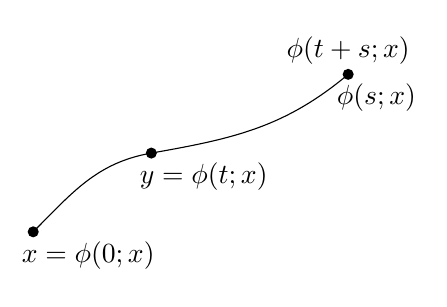
\begin{tikzpicture}
\coordinate (A) at (0,0);
\coordinate (B) at (1.5,1);
\coordinate (C) at (4,2);

\foreach \coor/\formula in {A/{x=\phi(0;x)},B/{y=\phi(t;x)},C/{\phi(s;x)}} {
  \fill (\coor) circle (2pt);
  \node[below right, inner xsep=-1ex] at (\coor) {$\formula$};
}
\node[above] at (C) {$\phi(t+s;x)$};
\draw (A) to[in=190] (B) to[out=10, in=220] (C);
\end{tikzpicture}
\end{document}